\documentclass[12pt]{article}

% Packages
\usepackage{lipsum}
\usepackage{setspace}
\usepackage{indentfirst}
\usepackage{geometry}
\usepackage[nonumberlist, toc]{glossaries}
\usepackage{graphicx}
\usepackage{caption}
\usepackage{subcaption}
\usepackage{tabularx}
\usepackage{booktabs}
\usepackage[numbered]{./latex/mcode}
\usepackage{enumitem}
\usepackage{xcolor}
\usepackage [autostyle, english = american]{csquotes}
\usepackage{fancyhdr}
\usepackage{amsmath}
\usepackage{cite}

% Formatting
\geometry{letterpaper, portrait, margin=.85in}

\pagestyle{fancy}
\lhead{MSXII Suspension Parameters}
\rhead{Midnight Sun Solar Car Team}

\MakeOuterQuote{"}

\begin{document}

% Title Ppage
\begin{titlepage}
	\vspace*{3cm}
	\centering
	
\includegraphics[width=.25\textwidth]{./LaTex/midnightSunLogoCircle.png}\par
	\vspace{1.5cm}
	{\scshape\LARGE Midnight Sun Solar Car Team \par}
	{\scshape\large University of Waterloo\par}
	\vspace{3.5cm}
	{\huge\bfseries MSXII Suspension Parameters\par}
	\vspace{0.2cm}
	\large Prepared for Project 3 of ME321 Winter 2017
	\vfill
	Prepared by:\par
	Devon Copeland\par
	\vspace{1cm}
	\today\par
\end{titlepage}

% Main Matter
\section{Background}
\subsection{Vehicle Design}
Midnight Sun Twelve (MSXII) is a cruiser class, solar electric vehicle being designed with the goal of competing in the 2018 American Solar Challenge (ASC 2018) and the 2019 World Solar Challenge (WSC 2019). By definition, cruiser class solar vehicles must be multi-occupant and are designed with the intent of being more practical than a typical, challenger class solar car. Because of the unique requirements of this class, the spring rates and target damping coefficients on MSXII's suspension must be selected to optimize for efficiency while still keeping driver comfort in mind. This report proposes an analytical technique for determining the response of a suspension system to any given road conditions. 

\subsection{Important Vehicle Parameters}
Table \ref{tab:params} lists vehicle parameters that are of importance to the design and analysis of MSXII's suspension. The mass and moment of inertia was computed by CAD software. 
\begin{table}[htbp]
	\centering
	\caption{Important Vehicle Parameters}
	\label{tab:params}
	\begin{tabular}{lll}
	Mass ($M$)                            	& 550  & $kg$       \\
	Wheelbase                       	 	& 2.60  & $m$  		\\
	Track                       	 		& 1.60  & $m$  		\\
	Distance from Front Wheel to CoG ($a$)	& 1.32 & $m$  		\\
	Distance from Road to CoG ($h$)		& 0.52 & $m$  		\\
	Moment of Inertia Normal to Symmetry Plane at CoG ($I_{xx}$) & 550  & $kgm^2$ \\
	Full Wheel Travel in Compression 	& 45   & $mm$ 		\\
	Front Coilover Angle from Vertical	& 40   & $\circ$ 	\\
	Rear Coilover Angle from Vertical	& 30   & $\circ$
	\end{tabular}
\end{table}
\subsection{Suspension Architecture}
MSXII's front suspension comprises of a double wishbone linkage with an outboard coilover while the rear suspension comprises of independent trailing arms allowing for zero scrub and thus less rolling resistance. Figure \ref{fig:solidworksScreenshots} shows the screenshots of the front and rear suspension.  
\begin{figure}[htbp]
	\centering
    \begin{subfigure}[b]{.32\textwidth}
		\caption{Front Isometric View}
		\centering
        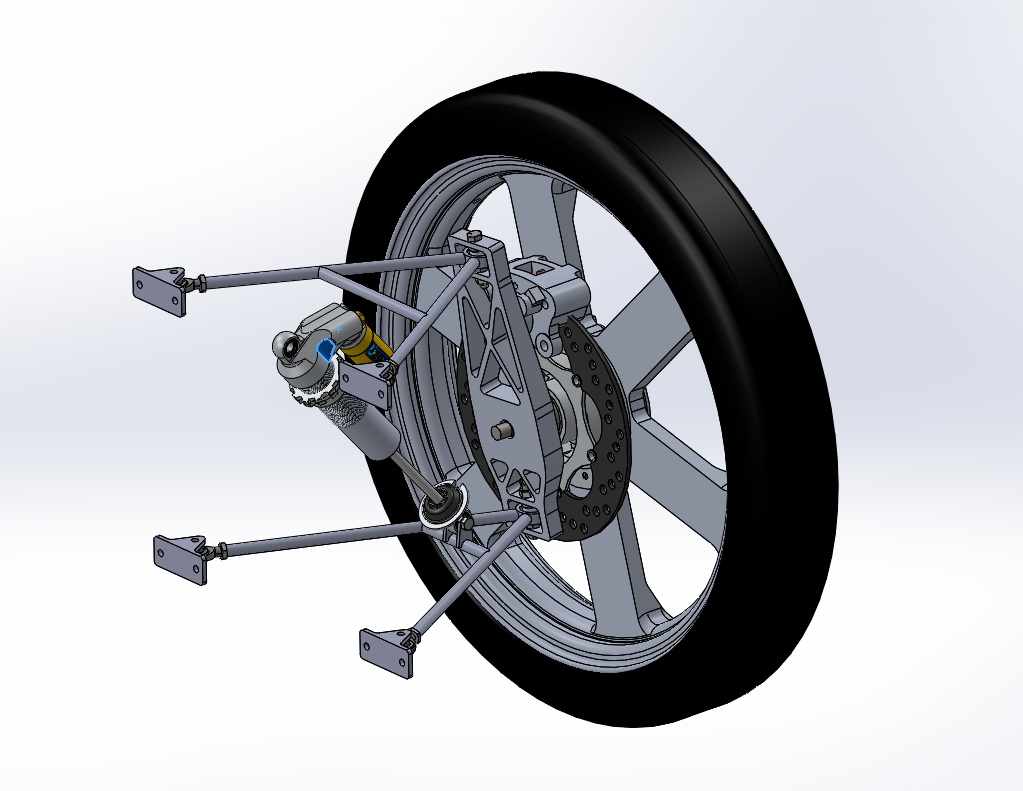
\includegraphics[height=3.5cm]{./LaTex/frontIso.PNG}
    \end{subfigure}
    \begin{subfigure}[b]{.32\textwidth}
		\caption{Rear Isometric View}
		\centering
        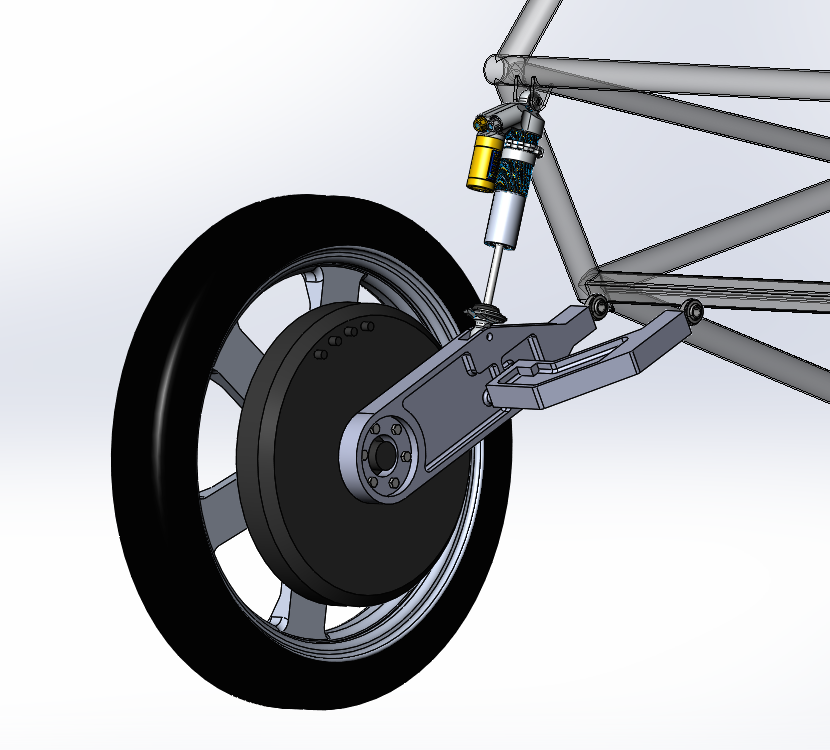
\includegraphics[height=3.5cm]{./LaTex/rearIso.PNG}
        \label{fig:c8}
    \end{subfigure}
    \begin{subfigure}[b]{.32\textwidth}
		\caption{Rear Sie View}
		\centering
        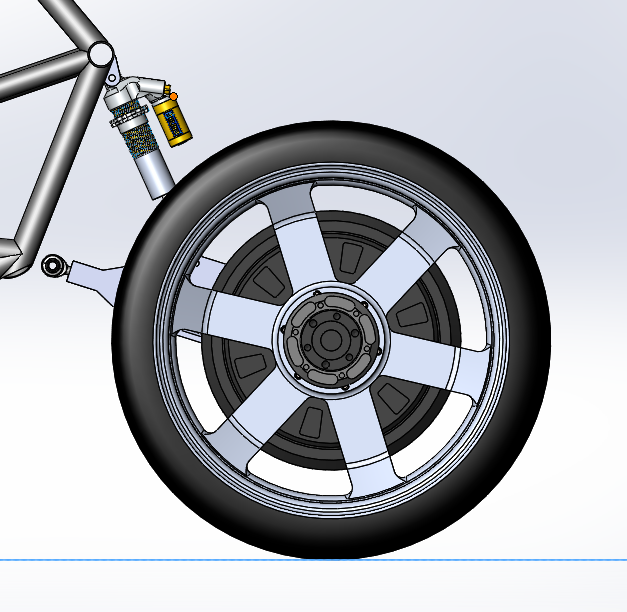
\includegraphics[height=3.5cm]{./LaTex/rearRight.PNG}
        \label{fig:c9}
    \end{subfigure}
    \caption{MSXII Suspension Design (Screenshots from Solidworks)}
	\label{fig:solidworksScreenshots}
\end{figure}
	
\subsection{Selecting Suspension Parameters}
\label{sec:paramSelection}
The spring rates are calculated based on the travel of the wheel and the maximum vertical loading of the wheel due to normal force from the road. Assuming a smooth driving surface, the largest normal force acting on the tire will occur while braking in a turn. To approximate this loading condition, the a superposition of two static half car models is used; one for cornering and one for hard braking.  
\subsubsection{Hard Braking}\begin{figure}[h!]
	\centering
	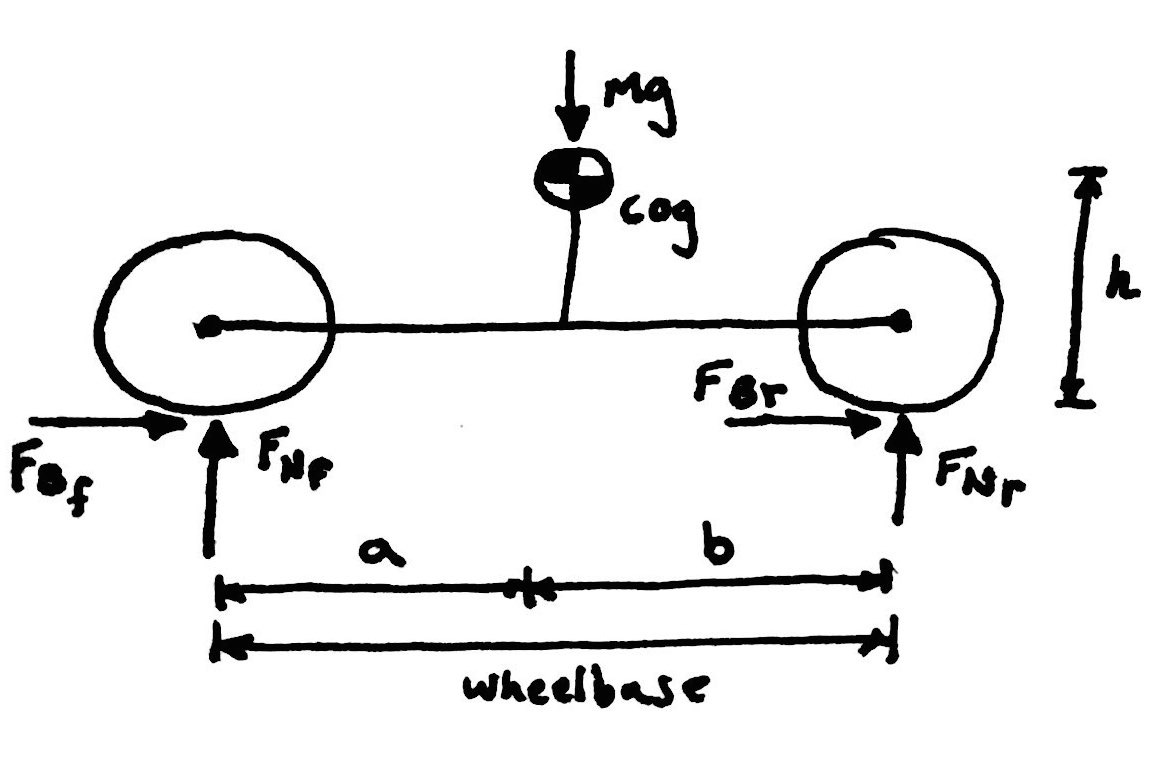
\includegraphics[width=.5\textwidth]{./LaTex/brakingFBD.jpg}
	\caption{Free Body Diagram of a Car Braking}
	\label{fig:barkingFBD}
\end{figure}
Figure \ref{fig:barkingFBD} shows a free body diagram of a half car model undergoing braking. MSXII will only have brake callipers on the front wheels however regenerative braking from the hub motors will also provide a braking force at the rear contact patches. Assuming a generous coefficient of static friction, $\mu _s$, of 1.0 and the extreme case where the both the font and rear tires are about to begin sliding, the combined braking force can be expressed as: 
\begin{equation}
	F_{braking} = F_{Nf} + F_{Nr} = \mu _s F_{N_{net}} =  \mu _s Mg = (1.0)(550kg)\left(9.81\frac{m}{s^2}\right) = 5.40kN
\end{equation}
From Figure \ref{fig:barkingFBD}, summing the moments about the centre of gravity and the vertical forces results in the following equations: 
\begin{equation}
	aF_{Nf} = hF_{braking} + bF_{Nr}
\end{equation}
\begin{equation}
	F_{Nf} + F_{Nr} = Mg
\end{equation}
Solving for the front normal force: 
\begin{equation}
\begin{split}
	aF_{Nf} &= hF_{braking} + b(Mg - F_{Nr})\\
	F_{Nf} &= \frac{hF_{braking} + bMg}{a+b} = \frac{(0.52m)(5.40kN)+(1.28m)(550kg)\left(9.81\frac{m}{s^2}\right)}{(1.32m)+(1.28m)} = 2.66kN
\end{split}
\end{equation}
Note that 2.66kN is for both front wheels. Therefore there is approximately \textbf{1.33kN} of normal force on each front tire during hard braking. 

\subsubsection{Cornering}
\begin{figure}[h!]
	\centering
	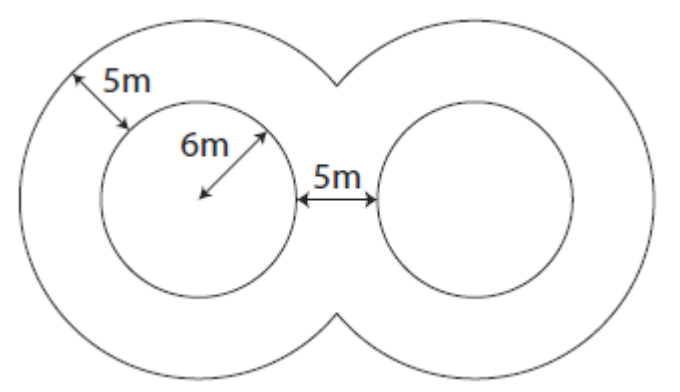
\includegraphics[width=.5\textwidth]{./LaTex/dynamicScrutineering.PNG}
	\caption{Figure of Eight Course from ASC 2018 Regulations 
	\cite{ASC2018regs}}
	\label{fig:dynamicScrutineering}
\end{figure}
The ASC 2018 regulations stipulate that a vehicle must be able to navigate a figure of eight as shown in Figure \ref{fig:dynamicScrutineering} in less than 18 seconds \cite{ASC2018regs}. Since the average arc length of the figure of eight is $34\pi m$, the net cornering force required to navigate the figure of eight can be found as follows:
\begin{equation}
	F_{si} + F_{so} = F_{steer} = \frac{Mv^2}{r} = \frac{(550kg)\left(\frac{34\pi m}{18s}\right)^2}{8.5m} = 2.28kN
\end{equation}
\begin{figure}[h!]
	\centering
	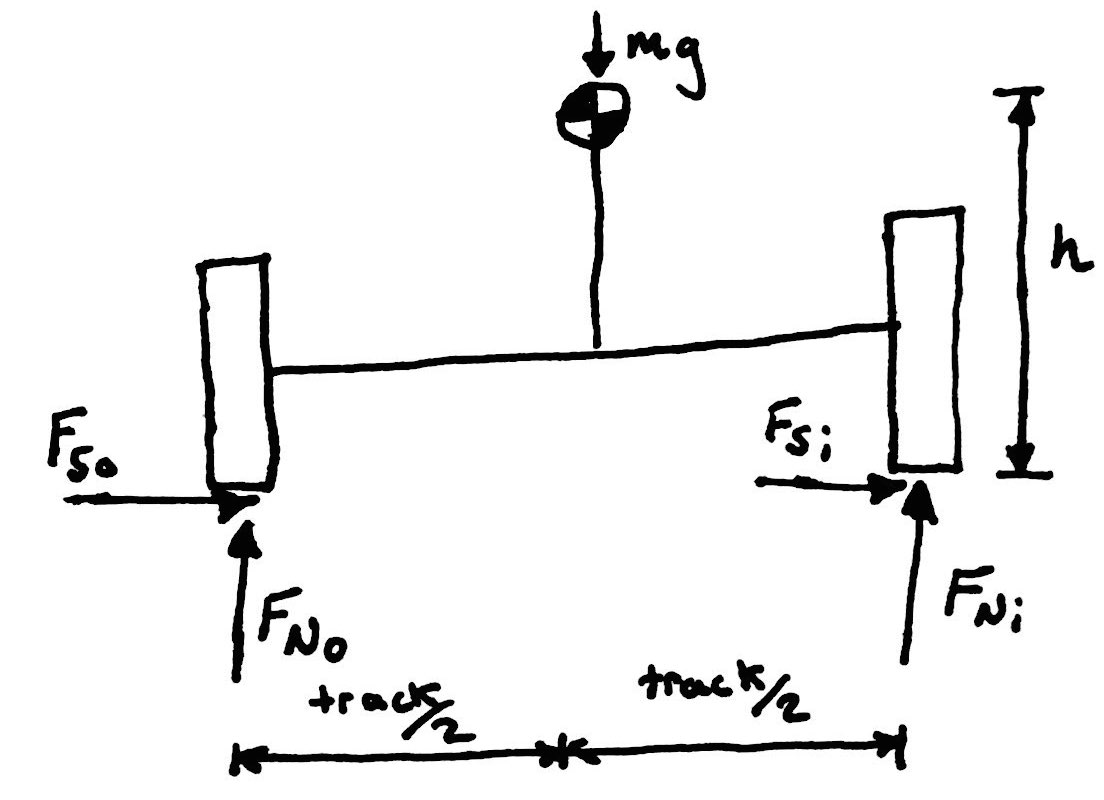
\includegraphics[width=.5\textwidth]{./LaTex/steerFBD.jpg}
	\caption{Free Body Diagram of a Car Cornering}
	\label{fig:steerFBD}
\end{figure}

\noindent For the half car model shown if Figure \ref{fig:steerFBD}, summing the moments about the centre of gravity and the vertical forces results in the following equations: 
\begin{equation}
	\frac{track}{2}F_{Nf} = hF_{steer} + \frac{track}{2}F_{Nr}
\end{equation}
\begin{equation}
	F_{No} + F_{Ni} = Mg
\end{equation}
Solving for the outside wheel normal force: 
\begin{equation}
\begin{split}
	\frac{track}{2}F_{No} &= hF_{steer} + \frac{track}{2}(Mg - F_{Ni})\\
	F_{No} &= \frac{hF_{steer} + \frac{track}{2}Mg}{track} = \frac{(0.52m)(2.28kN)+(0.80m)(550kg)\left(9.81\frac{m}{s^2}\right)}{1.60m} = 2.70kN
\end{split}
\end{equation}
Note that the 2.70kN above is for both front and rear outside wheels. Assuming the force is evenly split between the front and rear, there is approximately \textbf{1.35kN} of normal force on each outside tire during maximum cornering. 
\subsubsection{Spring Rate Selection}
Adding the maximum normal forces from cornering and braking results in 2.68kN. The maximum travel of the suspension for MSXII in compression has been set to 45mm. It is desired that under the combined loading condition of braking and cornering, the suspension compresses to a maximum of 70\% of the travel. As such, the desired spring rate is found to be: 
\begin{equation}
	k = \frac{force}{displacement} = \frac{2.68N}{(70\%)(0.045m)} = 85.0kN/m
\end{equation}
Note that the above rate assumes a vertical spring. The vertical spring rate can be mapped to an equivalent angled spring rate by dividing by the cosine of the angle that the coilover makes with the vertical direction: 
\begin{equation}
	\begin{split}
		k_{front} &= \frac{85.0}{cos(35)} = 110.6kN \\
		k_{rear} &= {85.0}{cos(30)} = 98.1kN
	\end{split}
\end{equation}
MSXII will be using Ohlins TTX25 MkII coilovers for both the front and rear. These coilovers can be configured to have spring rates from 150 lb/in to 650 lb/in in increments of 50 lb/in. 1 lb/in is approximately 175 N/m therefore 550 lb/in coils should be selected for the front and 650 lb/in coils for the rear. 

\subsubsection{Damping Coefficient Selection}
Ohlins has published damper curves for their TTX25 MkII's however real world damping rates are non constant. For this report, the damping coefficient will be idealized as constant and will be selected such that the damping ratio, $\zeta$, is 0.5. This is typical of high performance consumer vehicles \cite{dampers}. Given an equivalent vertical spring rate or 85.0kN/m, a damping ratio of 0.5 maps to a vertical damping coefficient of \textbf(4.83kNs/m). 

\section{Suspension Model}
\subsection{Overview}
MSXII's suspension is modelled using a point mass connected to two vertical, linear spring mass damper systems at the two wheels. This half car model assumes infinite tire stiffness and that the vehicle pitches about it's center of gravity. Figure \ref{fig:systemModel} describes the proposed model where: 
\begin{align*}
	\theta & \text{ is the pitch angle about the axis normal to the vehicle's symmetry plane}\\        
	x_0 & \text{ is the displacement of the center of gravity in the vertical axis} \\
	x_1 \text{ \& } x_2 & \text{ are the displacements of the mounting points for the front and rear wheels respectively} \\
	y_1 \text{ \& } y_2 & \text{ is the change in road elevation below the front  and rear wheels respectively} \\
	M & \text{ is the mass of the vehicle} \\
	I & \text{ is the moment of inertia normal to the vehicle’s symmetry plane at the center of gravity} \\
	k1,k2,c1 \text{ \& } c_2 & \text{ are the spring and damping coefficients} \\
	a \text{ \& } b & \text{ are the distances from center of gravity to the front and rear wheels respectively}
\end{align*}
\begin{figure}[h!]
	\centering
	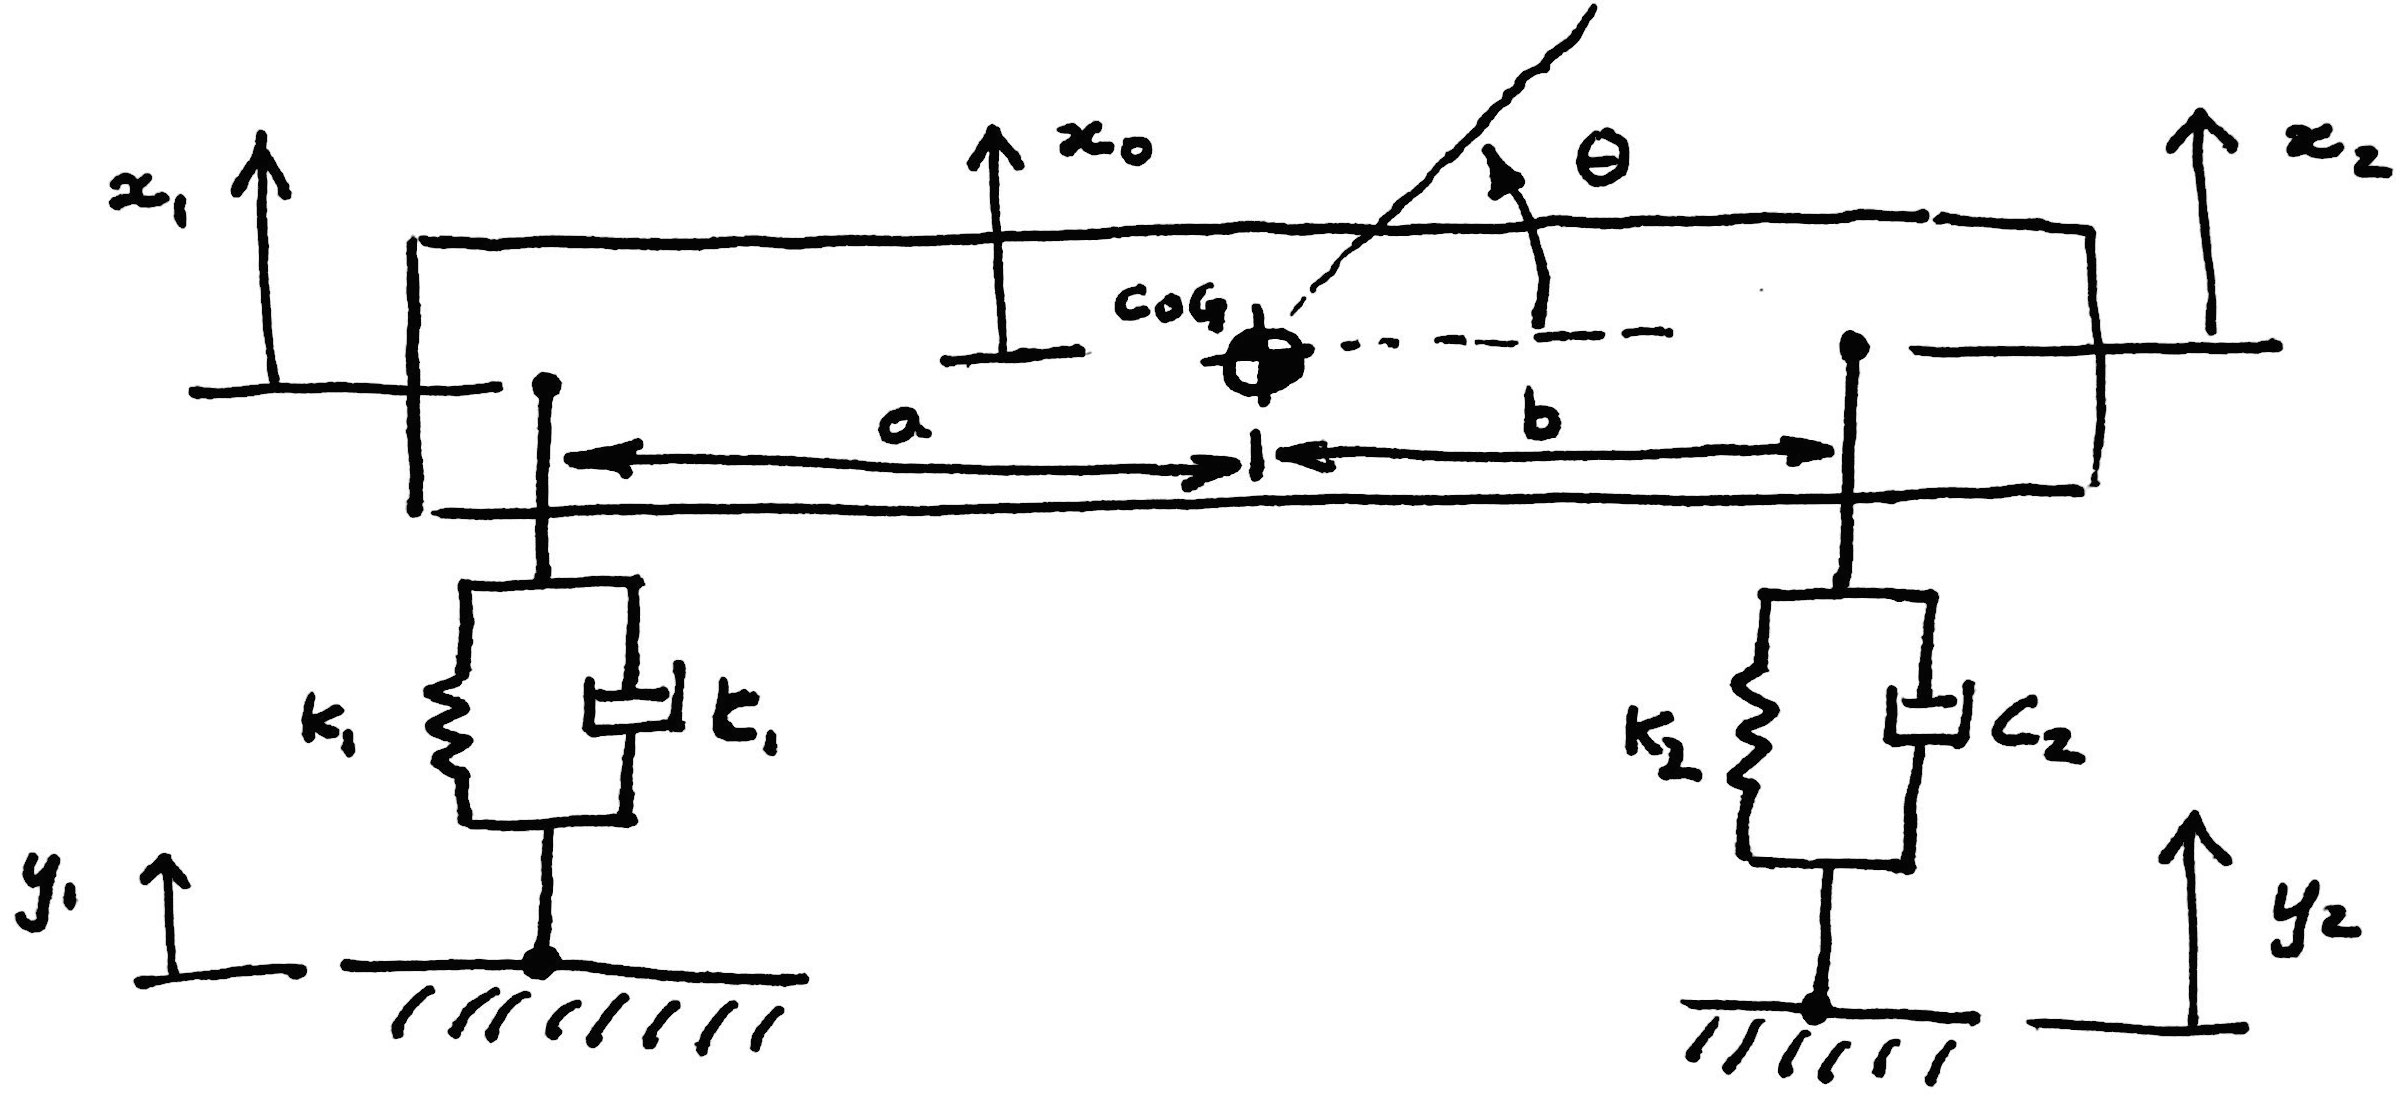
\includegraphics[width=.8\textwidth]{./LaTex/systemModel.jpg}
	\caption{Half car model with infinite tire stiffness}
	\label{fig:systemModel}
\end{figure}

\subsection{Equations of Motion}
\subsubsection{Dynamic Equilibrium}
The spring mass damper system shown in Figure \ref{fig:systemModel} can be described by the folowing two differential equations: 
\begin{equation}
	M \ddot x + c_1(\dot x_1 - \dot y_1) + c_2(\dot x_2 - \dot y_2) + k_1(x_1 - y_1) + k_2(x_2 - y_2) = 0
\end{equation}
\begin{equation}
	I \ddot\theta - ac_1(\dot x_1 - \dot y_1) + bc_2(\dot x_2 - \dot y_2) - ak_1(x_1 - y_1) + bk_2(x_2 - y_2) = 0
\end{equation}
Rearranging to move the inputs $y_1$ and $y_2$ to right hand side: 
\begin{equation}
	M \ddot x + c_1\dot x_1 + c_2\dot x_2 + k_1x_1 + k_2x_2 = c_1\dot y_1 + c_2\dot y_2 + k_1y_1 + k_2y_2
\end{equation}
\begin{equation}
	I \ddot\theta - ac_1\dot x_1 + bc_2\dot x_2 - ak_1x_1 + bk_2x_2 = -ac_1\dot y_1 + bc_2\dot y_2 - ak_1y_1 + bk_2y_2
\end{equation}
By assuming small pitch angles, $\theta$, the angle between the spring mass damper system becomes approximately perpendicular and the displacements $x_1$ and $x_2$ can be approximated as follows:
\begin{equation}
	x_1 = x_0 - a\theta
\end{equation}
\begin{equation}
	x_2 = x_0 + b\theta
\end{equation}
It follows that the time derivatives of the above two equations are: 
\begin{equation}
	\dot x_1 = x_0 - a\dot\theta
\end{equation}
\begin{equation}
	\dot x_2 = x_0 + b\dot\theta
\end{equation}
Substituting into the original differential equations: 
\begin{equation}
	M \ddot x + \dot x_0(c_2+c_1) + \dot\theta(bc_2-ac_1) + x_0(k_2+k_1) + \theta(bk_2-ak_1)= c_1\dot y_1 + c_2\dot y_2 + k_1y_1 + k_2y_2
\end{equation}
\begin{equation}
	I \ddot\theta + \dot x_0(bc_2-ac_1) + \dot\theta(b^2c_2+a^2c_1) + x_0(bk_2-ak_1) + \theta(b^2k_2+a^2k_1) = -ac_1\dot y_1 + bc_2\dot y_2 - ak_1y_1 + bk_2y_2
\end{equation}
The above two equations are considerably complex and are not particularly conducive of solving analytically by hand. However, the fact that the vehicle has the center of gravity approximately centered along the wheel such that $a$ and $b$ are equal, offers an avenue for simplification. Additionally if the front and rear spring and damping coefficients are assumed to be the same ($k$ and $c$ respectively), the problem's complexity is drastically reduced as shown in the following two equations: 
\begin{equation}
	M \ddot x + 2c\dot x_0 + 2kx_0 = c\dot y_1 + c\dot y_2 + ky_1 + ky_2
\end{equation}
\begin{equation}
	I \ddot\theta + 2a^2c\dot\theta + 2a^2k\theta = -ac\dot y_1 + bc_2\dot y_2 - ak_1y_1 + bk_2y_2
\end{equation}

\subsubsection{Natural Frequency}
The natural frequency of the translational and rotational components of the system are found as follows: 
\begin{equation}
	\begin{split}
	\omega _{nx} &= \sqrt{\frac{k_{eq}}{m_{eq}}} = \sqrt{\frac{2k}{M}}\\
	\omega _{n\Theta} &= \sqrt{\frac{k_{eq}}{m_{eq}}}= \sqrt{\frac{2a^2k}{I}}
	\end{split}  
\end{equation}

\subsubsection{Critical Damping}
The critical camping coefficient for the translational and rotational components of the system are found as follows:
\begin{equation}
	\begin{split}
	c_{eqx} = 2c, c_{rx} = 2m_{eq}\omega _n = \sqrt{8kM}, \zeta _x = \frac{c_{eqx}}{c_r}\\
	c_{eq\Theta} = 2a^2c, c_{r\Theta} = 2m_{eq}\omega _n = \sqrt{8a^2kI}, \zeta _\Theta = \frac{c_{eq\Theta}}{c_r}
	\end{split}  
\end{equation}

\subsubsection{Final Equations of Motion}
The road displacement can be approximated by a sinusoid with and amplitude $A$ and a base excitation frequency $\omega _b$. Since the rear wheels experience the same displacements as the front $y_2$ can be expressed as a phase shifted version of $y_1$. Combining this with the natural frequency and damping ratio results in the following equations of motion: 
\begin{equation}
	\label{eq:eomx}
	\ddot x + (2\zeta _x M \omega _{nx}) \dot x_0 + (\omega _{nx}^2)x_0 = \frac{cA\omega _b}{M}cos(\omega _b t) + \frac{cA\omega _b}{M}cos(\omega _b (t-t_0))  + \frac{kA}{M}sin(\omega _b t) + \frac{kA}{M}sin(\omega _b (t-t_0))
\end{equation}
\begin{equation}
	\label{eq:eomtheta}
	\begin{split}
		\ddot\theta + &(2\zeta _\Theta  I \omega _{n\Theta}) \dot\theta + (\omega _{n\Theta}^2)\theta \\&= -\frac{acA\omega _b}{I}cos(\omega _b t) + \frac{acA\omega _b}{I}cos(\omega _b (t-t_0)) - \frac{kcA\omega _b}{I}sin(\omega _b t) + \frac{akA\omega _b}{I}sin(\omega _b (t-t_0))
	\end{split}
\end{equation}

\subsection{Total Response}
\subsubsection{Base Excitation Parameters}
To model real road conditions, a sinusoid with a amplitude of 0.015 and a frequency of 69.7 rad/s is used. This corresponds to 30mm peak to peak bumps that are separated by a distance of 2m while driving at 80km/hr (calculated in Appendix \ref{app:simple}). 

\subsubsection{Initial conditions}
For the total response, the initial conditions of the system are all set to zero. This represents the vehicle traveling on a perfectly smooth road before encountering disturbances at time $t = 0$. 

\subsubsection{Solution}
Based on the idealize parameters proposed in Section \ref{sec:paramSelection} , the natural frequency and damping ratio are found as follows: 
\begin{equation}
	\begin{split}
	\omega _{nx} &= \sqrt{\frac{2k}{M}} = \sqrt{\frac{(2)(85000N/m)}{550kg}} = 17.58rad/s = 2.80Hz \\
	\omega _{n\Theta} &= \sqrt{\frac{2a^2k}{I}} = \sqrt{\frac{(2)(1.3^2m^2)(85000N)}{550kgm^2}} = 22.86rad/s = 3.64Hz 
	\end{split}  
\end{equation}
\begin{equation}
	\begin{split}
		c_{eqx} &= 2c = (2)(4830Ns/m) = 9660Ns/m \\ 
		c_{rx} &= 2M\omega _n = (2)(550kg)(17.58rad/s) = 19340Ns/m \\ 
		\zeta _x& = \frac{c_{eqx}}{c_r} = \frac{9660Ns/m}{19340Ns/m} = 0.50\\
		c_{eq\Theta} &= 2a^2c =  2(1.3^2m^2)(4830Ns/m) = 16330Nms\\
		c_{r\Theta} &= 2m_{eq}\omega _n = (2)(550kgm^2)(22.86rad/s) = 25150Nms\\ 
		\zeta _\Theta &= \frac{c_{eq\Theta}}{c_r} = \frac{16330Nms}{ 25150Nms} = 0.65
	\end{split}  
\end{equation}
Using the MATLAB script shown in Appendix \ref{app:simple}, values for the parameters $I$, $M$, $k$, $c$, and $a$ are substituted into Equations \ref{eq:eomx} and \ref{eq:eomtheta} and the Laplace transform is taken. Solving for $X(s)$ and $\Theta(s)$ and taking the inverse Laplace transform yeilds:
\begin{equation}
		\begin{split}
		x(t) = &(3.12\cdot 10^{-5})\, \sin\!(69.7\, t) - 0.00201\, \cos\!(69.7\, t) + 1.0\, \mathop{\mathrm{u}}\nolimits\!(1.0\, t - 0.117)\, ((5.91\cdot 10^{-4})\, \cos\!(69.7\, t) \\
		&- 0.00192\, \sin\!(69.7\, t)) + \mathrm{e}^{- 8.78\, t}\, (0.00201\, \cos\!(15.2\, t) + 0.00102\, \sin\!(15.2\, t) \\
		&- \mathop{\mathrm{u}}\nolimits\!(1.0\, t - 0.117)\, (0.00396\, \cos\!(15.2\, t) - 0.00489\, \sin\!(15.2\, t)))
		\end{split}
\end{equation} 

\begin{equation}
\begin{split}
	\theta (t) =& 0.00242\, \cos\!(69.7\, t) + (3.31\cdot 10^{-4})\, \mathop{\mathrm{u}}\nolimits\!(1.0\, t - 0.117)\, \cos\!(69.7\, t) - 0.00242\, \mathrm{e}^{- 14.8\, t}\, \cos\!(9.42\, t) \\
	 &- (5.64\cdot 10^{-4})\, \mathrm{e}^{- 14.8\, t}\, \sin\!(9.42\, t) - 1.0\, \sin\!(69.7\, t)\, (0.00244\, \mathop{\mathrm{u}}\nolimits\!(1.0\, t - 0.117) + 4.39\cdot 10^{-4}) \\
	 &+ 0.00334\, \mathop{\mathrm{u}}\nolimits\!(1.0\, t - 0.117)\, \mathrm{e}^{- 14.8\, t}\, \cos\!(9.42\, t) + 0.0137\, \mathop{\mathrm{u}}\nolimits\!(1.0\, t - 0.117)\, \mathrm{e}^{- 14.8\, t}\, \sin\!(9.42\, t)
\end{split}
\end{equation}

\subsubsection{Plotting Total Response}
Figure \ref{fig:totalResp} shows the total response of the system subjected to the simulated road input. 
\begin{figure}[h!]
	\centering
	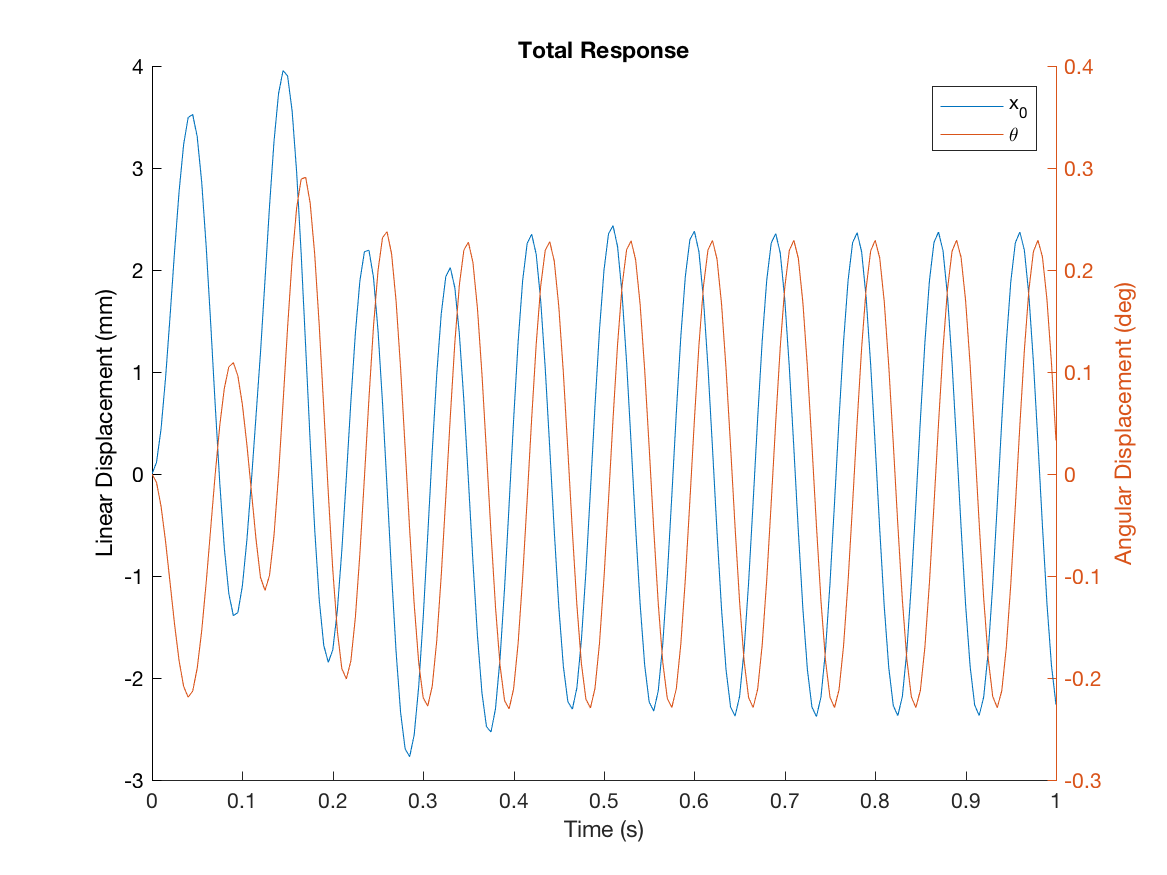
\includegraphics[width=.8\textwidth]{./matlab/totalResp.png}
	\caption{Total Response of the System}
	\label{fig:totalResp}
\end{figure}


\subsection{Alternate Formulation}
If the center of gravity is not centered between the front and rear wheel axes, the problem increases significantly in complexity and an alternate approach to solving the problem is required. By taking the unilateral Laplace transform of the above two equations with all initial conditions set to zero, the following $s$ domain equations are obtained:
\begin{equation}
	\left[Ms^2+(c_2+c_1)s+(k_2+k_1)\right]X_0 + \left[(bc_2-ac_1)s+(bk_2+ak_1)\right]\Theta = c_1sY_1 + c_2sY_2 + k_1Y_1 + k_2Y_2
\end{equation}
\begin{equation}
	\left[(bc_2-ac_1)s+(bk_2-ak_1)\right]X_0 + \left[Is^2+ (b^2c_2+a^2c_1)s+(b^2k_2+a^2k_1)\right]\Theta = c_1sY_1 + c_2sY_2 + k_1Y_1 + k_2Y_2
\end{equation}
The above two equations can be expressed in matrix form as follows: 
\begin{equation}
	\label{eq:matrix1}
	\begin{bmatrix} 
	Q_{Ax}(s) & Q_{A\Theta}(s) \\
	Q_{Bx}(s) & Q_{B\Theta}(s)
	\end{bmatrix}
	\begin{bmatrix} 
	X_0 \\
	\Theta 
	\end{bmatrix}
	= 
	\begin{bmatrix} 
	P_{A1}(s) \\
	P_{B1}(s)
	\end{bmatrix}Y_1 +
	\begin{bmatrix} 
	P_{A2}(s) \\
	P_{B2}(s)
	\end{bmatrix}
	Y_2
\end{equation}
If it is assumed that the rear tire of the car experiences the exact same road conditions as the front tire, $Y1$ and $Y2$ can be expressed as functions of the same input, $Y$ where $Y2$ is simply a phase shifted version of $Y1$:
\begin{equation}
	\begin{split}
		y_1(t) &= y(t)\\
		y_2(t) &= y(t-t_0)
	\end{split} \implies
	\begin{split}
		Y_1(s) &= Y(s)\\
		Y_2(s) &= Y(s)e^{-st_0}
	\end{split}
\end{equation}
Equation \ref{eq:matrix1} can then be rewritten as follows:
\begin{equation}
	\label{eq:matrix1}
	Q
	\begin{bmatrix} 
	X_0 \\
	\Theta 
	\end{bmatrix}
	= 
	\left(\left[P_1\right]+\left[P_2\right]e^{-st_0}\right)Y
\end{equation}
Since the system is linear, the above matrix equation can be solved in two parts to obtain the transfer functions for $X_0$ and $\Theta$:
\begin{equation}
	\frac{\begin{bmatrix} 
		X_0 \\
		\Theta 
	\end{bmatrix}}{Y} =
	\left[H\right] = 
	\left[H_1\right] + \left[H_2\right] = 
	[Q^{-1}][P_1] + [Q^{-1}][P_1]e^{-st_0} 
\end{equation} 

Using the MATLAB script shown in Appendix \ref{app:alternative}, the transfer function $H(s)$ is solved for symbolically as described above and the parameters for $I$, $M$, $k_1$, $k_2$, $c_1$, $c_2$, $a$ and $b$ are substituted into the equation. The inverse laplace transform is then taken to obtain the impulse response as shown in Figure \ref{fig:impResp}.
\begin{figure}[h!]
	\centering
	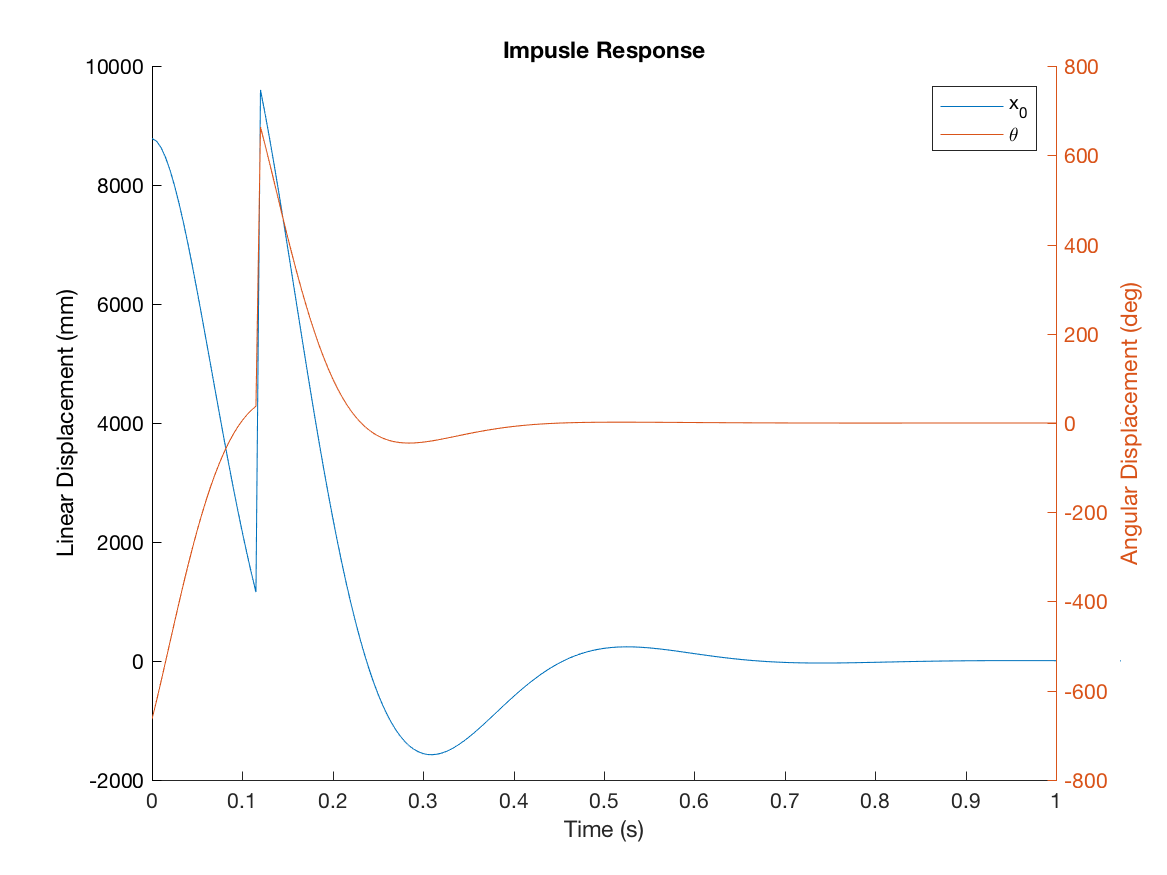
\includegraphics[width=.8\textwidth]{./matlab/impResp.png}
	\caption{Undamped Impulse Response}
	\label{fig:impResp}
\end{figure}

By performing an Fast Fourier Transform on the undamped system the harmonics of the system can be approximated as shown in Figure \ref{fig:fftImpResp}. A sampling frequency of 200Hz and and a window of 30s was used for the FFT.
\begin{figure}[h!]
	\centering
	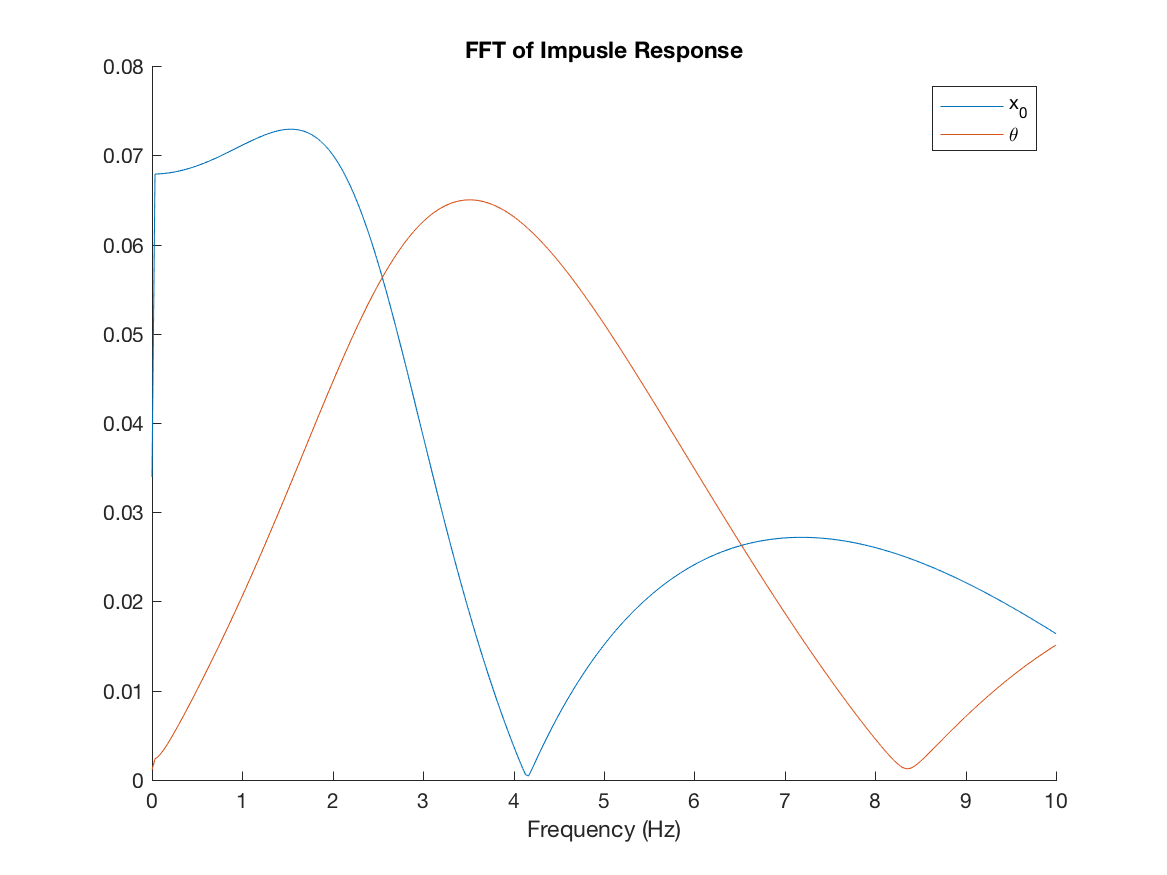
\includegraphics[width=.8\textwidth]{./matlab/fftImpResp.png}
	\caption{FFT of the Undamped Impulse Response}
	\label{fig:fftImpResp}
\end{figure}
From Figure \ref{fig:fftImpResp}, the largest harmonics of the system occur at approximately 2Hz for translational displacement and 4Hz for angular displacement. Note that these frequencies align closely with the natural frequencies that were determined analytically in the simplified case.  

% Source
\pagebreak
\bibliography{bib}{}
\bibliographystyle{plain}

% Appendix
\pagebreak
\appendix
\section{MATLAB Source Code for Simplified Model}
\label{app:simple}
\lstinputlisting[breaklines=true]{./matlab/alternativeFormulation.m}
\pagebreak
\section{MATLAB Source Code for Alternative Formulation}
\label{app:alternative}
\lstinputlisting[breaklines=true]{./matlab/simplifiedFormulation.m}

\end{document}